\documentclass[a4paper]{article}
\usepackage[utf8]{inputenc}
\usepackage{fullpage}
\usepackage{csquotes}
\usepackage[ngerman]{babel}
\usepackage{biblatex}
\usepackage{float}
\usepackage{graphicx}
\usepackage{subfigure}
\usepackage[format=plain,labelfont=bf,up]{caption}
\usepackage{hyperref}
\bibliography{documentation.bib}
\title{Impaired Vision \\ Ein Augmented-Reality-Simulator für Sehstörungen}
\author{Willi Schönborn}
\date{\today}
\begin{document}

\begin{figure}[H]
\centering

\includegraphics{beuth.png}
\maketitle
\end{figure}

\section*{Einleitung}
Als Teil der Lehrveranstaltung \textit{Multimediatechnik Vertiefung} an der \textit{Beuth Hochschule für Technik Berlin} soltel im Rahmen einer Semesterarbeit ein Projekt mit Bezügen zu den Bereichen Multimedia und Wahrnehmung entstehen. Das Ziel dieses Dokumentes ist es die Ideen, Konzepte sowie die Ergebnisse dieses Projektes vorzustellen.

\section*{Augmented Reality}
Unter \textit{Augmented Reality} versteht man die computergestützte Erweiterung der Realitätswahrnehmung \cite{WP-AR}. Es gibt diverse doch sehr ausschweifende Definitionen dieses Begriffs. Innerhalb dieses Dokumentes wird Augmented Reality als die visuelle Darstellung von Informationen verstanden, also die Ergänzung von Bildern oder Videos mit computergenerierten Zusatzinformationen oder virtuellen Objekten mittels Einblendung/Überlagerung \cite{WP-AR}. Abbildung \ref{augmented-reality} zeigt eine typische Anwendung der Prinzipien von Augmented Reality anhand einer Anwendung für Smartphones, die es erlaubt geographische Informationen über Objekte die sich im Sichtfeld des Betrachters befinden direkt über das Kamerabild zu legen. Mithilfe solcher Augmented-Reality-Anwendungen entsteht eine neuartige Wahrnehmung der Umgebung. Genau an dieser Stelle setzt die Idee dieses Projektes an: Eine ungewohnte Sicht auf gewohnte Dinge ermöglichen.

\begin{figure}[H]
\centering
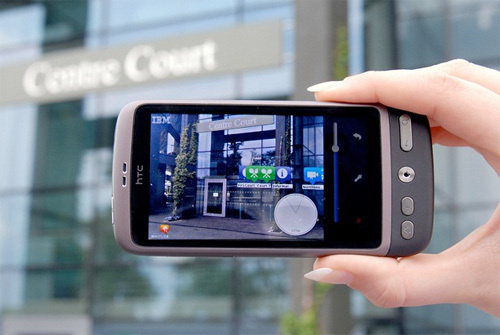
\includegraphics[width=\textwidth, trim=0 50 0 60, clip=true]{augmented-reality.jpg}
\caption{Augmented Reality Anwendung}
\label{augmented-reality}
\end{figure}

\newpage

\section*{Idee}
Das Ergebnis dieses Projektes sollte ein Anwendung für Mobiltelefone werden, die es ermöglicht diverse Sehstörungen für normalsichtige Menschen zu simulieren. In der schriftlichen Projektidee wurden als mögliche Kandidaten für die Sehstörungen, die simuliert werden können Rot-Grün-Sehschwäche, Gelb-Blau-Sehschwäche sowie Kurzsichtigkeit aufgeführt. Nach einigen Recherchen sowie dem ausgiebigen Studium von \textit{Sensation and Perception} \cite{Goldstein2009} wurde relativ schnell deutlich, dass umgangssprachliche Vereinfachungen wie \textit{farbenblind} oder \textit{Rot-Grün-Schwäche} differenzierter betrachtet werden müssen um zu einem zufriedenstellenden Projektergebis zu kommen. Zu diesem Zweck werden im nächsten Kapitel alle Sehstörungen näher behandelt und analysiert, die später simuliert werden sollen.

\section*{Sehstörungen}
Insgesamt wurden fünf unterschiedliche Sehschwächen ausgewählt wobei der Schwerpunkt klar auf den Farbfehlsichtigkeiten liegt. Neben der klassischen Myopie, der Kurzsichtigkeit, sowie den drei Vertretern der Dichromasie, der teilweisen Farbblindheit \cite{WP-D} wird auch die Achromasie, die komplette Farbenblindheit, behandelt. Alle modifizierten Versionen der Beispielabbildungen in diesem Kapitel wurden mithilfe von Vischeck \cite{VISCHECK} erzeugt.

\subsection*{Myopie}
Kurzsichtigkeit oder Myopie bezeichnet man eine bestimmte Form von optischer Fehlsichtigkeit bei der ein Missverhältnis zwischen Baulänge und Brechkraft des Auges besteht. Das Ergebnis ist ein Abbildungsfehler, der weit entfernte Objekte unschärfer erscheinen lässt als nahe gelegene. Der Betroffene sieht also in der Ferne schlechter als in der Nähe \cite{WP-KS}. Abbildung \ref{myopia} verdeutlicht den Effekt anhand eines Fotos, das mit meinem Gauß-Filter modifiziert wurde. Die physikalische Grundlage ist hier nicht absolut korrekt, da bei der Kurzsichtigkeit natürlich die Entfernung eine große Rolle spielt, bei zunehmend großen Distanzen kann diese Tatsache jedoch vernachlässigt werden.

\begin{figure}[H]
\centering
\subfigure[Normalsichtigkeit]{
    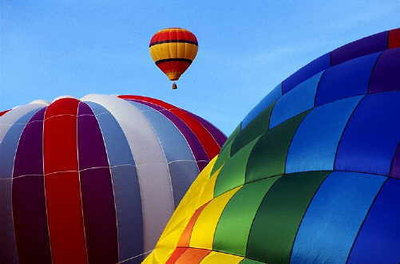
\includegraphics[width=0.48\textwidth]{balloons.jpg}
}
\subfigure[Myopie (Kurzsichtigkeit)]{
    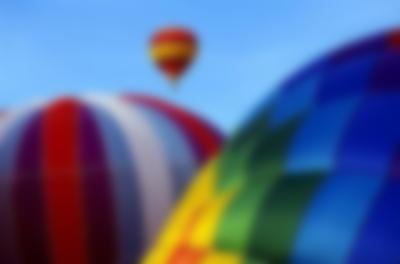
\includegraphics[width=0.48\textwidth]{balloons-myopia.jpg}
}
\caption{Myopie im Vergleich}
\label{myopia}
\end{figure}

\newpage

\subsection*{Protanopie}
Protanopie, oder auch Rotblindheit, ist einer Art der Dichromasie, also eine Farbsehstörung bei der nur zwei der drei Zapfen-Arten funktionsfähig sind. Bei Menschen mit Protanopie unterscheiden sich rote und grüne Zapfen nicht mehr in ihrer Farbantwort. Protanope haben daher nur zwei statt drei verschiedene Zapfentypen. Betroffen sind etwa 1 \% der Männer und 0,02 \% der Frauen. Im kurzwelligen Bereich sehen sie ein sattes Blau, im mittelwelligen Bereich Grau und im langwelligen Bereich ein sattes Gelb \cite{WP-P}.

\begin{figure}[H]
\centering
\subfigure[Normalsichtigkeit]{
    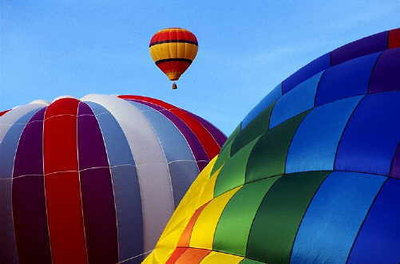
\includegraphics[width=0.48\textwidth]{balloons.jpg}
}
\subfigure[Protanopie]{
    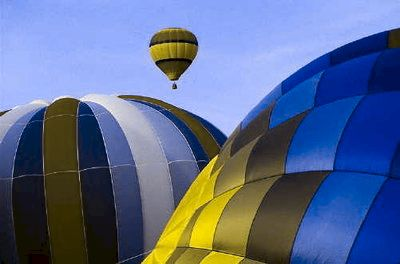
\includegraphics[width=0.48\textwidth]{balloons-protanope.jpg}
}
\caption{Protanopie im Vergleich}
\label{protanope}
\end{figure}

\subsection*{Deuteranopie}
Auch bei der Deuteranopie, oder Gründblindheit, handelt sich dabei um eine genetisch bedingte Farbfehlsichtigkeit Deuternaropen haben jedoch, im Gegensatz zu Protanopen, keine funktionsfähigen M-Zapfen da die Zapfen für das Wahrnehmen von Grün das Opsin für Rot enthalten \cite{WP-D}. Die Krankheitshäufigkeit von Deuteranopie liegt im selben Bereich wie die der Protanopie. Interessant ist die Tatsache, dass beide Krankheiten, sowohl die Rot- als auch die Grünblindheit, einen ausgesprochen ähnlichen visuellen Effekt ergeben. Betroffene können in beiden Fällen Rot- und Grüntöne der gleichen Helligkeit nicht mehr auseinanderhalten. Aus diesem Grund werden beide Krankheiten oft unter dem Begriff Rot-Grün-Sehschwäche zusammengefasst. Die Abbildung \ref{protanope} und \ref{deuteranope} zeigen die jeweiligen Symptome im direkten Vergleich mit der Normalsichtigkeit.

\begin{figure}[H]
\centering
\subfigure[Normalsichtigkeit]{
    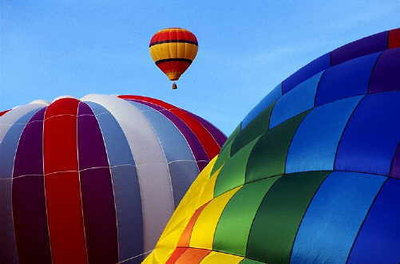
\includegraphics[width=0.48\textwidth]{balloons.jpg}
}
\subfigure[Deuteranopie]{
    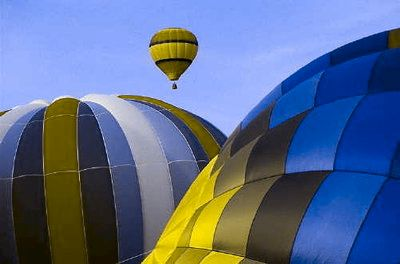
\includegraphics[width=0.48\textwidth]{balloons-deuteranope.jpg}
}
\caption{Deuteranopie im Vergleich}
\label{deuteranope}
\end{figure}

\newpage

\subsection*{Tritanopie}
Tritanopie, oder Blaublindheit, bezeichnet eine genetisch bedingte Farbfehlsichtigkeit, bei der den Betroffenen die Blau-Zapfen in der Retina fehlen \cite{WP-T}. Die Prävalenz von Tritanopie ist mit etwa 0,002 \% der Männer und 0,001 \% der Frauen verglichen mit Protanopie und Deuteranopie deutlich geringer. Die Tatsache, dass Betroffene keine Funktionsfähigen S-Zapfen haben führt dazu, dass mittlere und kurze Wellenlängen nicht mehr einwandfrei unterschieden werden können. Abbildung \ref{tritanope} verdeutlicht diesen Effekt.

\begin{figure}[H]
\centering
\subfigure[Normalsichtigkeit]{
    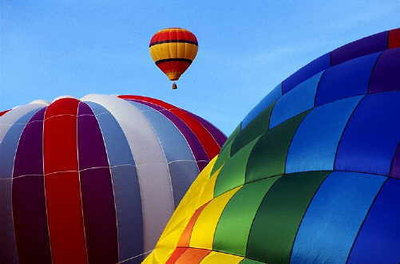
\includegraphics[width=0.48\textwidth]{balloons.jpg}
}
\subfigure[Tritanopie]{
    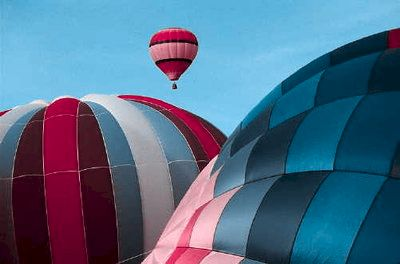
\includegraphics[width=0.48\textwidth]{balloons-tritanope.jpg}
}
\caption{Tritanopie im Vergleich}
\label{tritanope}
\end{figure}

\subsection*{Achromasie}
Die Farbenblindheit, Achromatopsie oder Achromasie ist eine seltene Farbsinnstörung, bei der keine Farben, sondern nur Hell-Dunkel-Kontraste wahrgenommen werden können. Bei Achromaten funktioniert keine der drei Zapfenarten, sie können somit keine Farben erkennen \cite{WP-A}. Neben der Unfähigkeit Farben zu erkennen leiden Achromaten zusätzlich darunter, dass im Bereich der Fovea keinerlei funktionierende Rezeptoren existieren. Dadurch fehlt ein Großteil der Sehschärfe. Abbildung \ref{achromate} versucht den visuellen Effekt mithilfe eines Graustufenbildes und eines Gauß-Filters zu simulieren. Allerdings lässt sich der visuelle Eindruck für Normalsichtige nicht zuverlässig darstellen. Diese Abbildung sollte deshalb nur als mögliche Interpretation verstanden werden.

\begin{figure}[H]
\centering
\subfigure[Normalsichtigkeit]{
    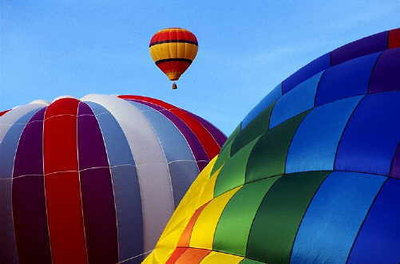
\includegraphics[width=0.48\textwidth]{balloons.jpg}
}
\subfigure[Achromasie]{
    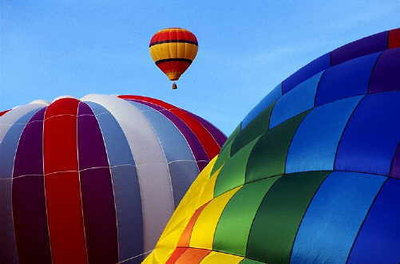
\includegraphics[width=0.48\textwidth]{balloons-achromate.jpg}
}
\caption{Achromasie im Vergleich}
\label{achromate}
\end{figure}

\newpage

\section*{Implementierung}

\newpage

\nocite{WP-RG}
\nocite{WP-GF}
\nocite{ANDROID}
\nocite{GIZMODO}
\nocite{IBFB}
\printbibliography

\listoffigures

\end{document}

